\section{Grundlagen}

\subsection{Grammatikkompression}

\begin{frame}
    \frametitle{Grammatikkompression}
	
	\note[item] {CFG: Wahrscheinlich keine große Erklärung nötig}
	\note[item] {Immer ein Nichtterminal auf beliebigen String aus Terminalen und Nichtterminalen}
	\note<2->[item] { 
		Grammatikkompression
		\begin{itemize}
			\item Eingabestring $s$ aus Alphabet $\Sigma$
			\item Grammatik erzeugt nur Eingabestring
			\item möglichst klein $\rightarrow$ muss noch kodiert werden, aber nicht Teil der Arbeit. Ausblick
		\end{itemize}
	}
	\note<3->[item]{kleinste Grammatik ist NP-Vollständig.}
	\note<3->[item]{Also nur approximative Lösung.}

	\begin{block}{Kontextfreie Grammatik}<1->
        Grammatik $G = (N, \Sigma, P, S)$ mit Nichtterminalen $N$, Terminale $\Sigma$ (auch \textit{Alphabet}), einer Startregel $S \in N$ und Produktionsregeln $P$.
		
        Die Regeln in $P$ haben die Form $X \rightarrow w$, wobei $X \in N$ und $w \in (N \cup \Sigma)^*$.
    \end{block}


    \begin{block}{Grammatikkompression}<2->
        Sei $s \in \Sigma^*$ ein String über das Alphabet $\Sigma$. 

        Generiere eine möglichst kleine kontextfreie Grammatik $G$, dessen Sprache $L(G) = \{s\}$ ist. (= Straight-Line-Grammatik)
    \end{block}

	\begin{itemize}
		\item<3->[$\Rightarrow$] Berechnung kleinster Grammatik $\mathcal{NP}$-vollständig \cite{charikar_smallest_2005}
	\end{itemize}
\end{frame}

\begin{frame}
	\frametitle{Größe einer Grammatik}

	\note[item]{Größe einer Grammatik definiert als die Summe der Länge aller rechten Seiten der Produktionsregeln}
	\note[item]{Gesamtanzahl der Zeichen in allen rechten Seiten}

	\begin{block}{Größe einer Grammatik}
		Für eine Grammatik $G = (N, \Sigma, P, S)$ ist die Größe definiert als
		\begin{equation*}
			|G| := \sum_{(A \rightarrow \alpha) \in P} |\alpha|.
		\end{equation*}
		Also die Summe der Länge aller rechten Seiten der Produktionsregeln.
	\end{block}

\end{frame}

\begin{frame}
	\frametitle{Tiefe einer Straight-Line-Grammatik}

	\note[item]{Als nächstes: Tiefe der Grammatik}
	\note[item]{Definiert als die Höhe ihres Ableitungsbaums \begin{itemize}
		\item Ableitungsbaum ist eindeutig weil: \begin{itemize}
			\item Definiert für Straight-Line-Grammatiken 
			\item Sprache besteht also nur aus einem Wort
			\item Grammatik ist so konstruiert, dass nur ein Ableitungsbaum möglich ist
		\end{itemize}
	\end{itemize}}
	\note<2->[item]{Beispiel \begin{itemize}
		\item Grammatik
		\item Ableitungsbaum
		\item<3-> Höhe 4
	\end{itemize}}

	\begin{block}{Tiefe einer Straight-Line-Grammatik}
		Die Tiefe einer Straight-Line-Grammatik ist definiert als die Höhe ihres Ableitungsbaums.
	\end{block}

	\begin{exampleblock}<2->{Beispiel}
		
		\begin{columns}
			\begin{column}{0.2\linewidth}
				$\begin{aligned}
					S &\rightarrow AB\\
					A &\rightarrow ab\\
					B &\rightarrow cC\\
					C &\rightarrow de
				\end{aligned}$
			\end{column}
			\begin{column}{0.45\linewidth}
				\centering
				\begin{tikzpicture}
					\node (S) at (0,0) {S};
					\node (A) at (-0.7, -0.7) {A};
					\node (ab) at (-0.7, -1.4) {ab};
					\node (B) at (0.7, -0.7) {B};
					\node (c) at (0, -1.4) {c};
					\node (C) at (1.4, -1.4) {C};
					\node (de) at (1.4, -2.1) {de};
	
					\draw (S) -- (A);
					\draw (S) -- (B);
					\draw (A) -- (ab);
					\draw (B) -- (c);
					\draw (B) -- (C);
					\draw (C) -- (de);
				\end{tikzpicture}
			\end{column}
			\begin{column}<3>{0.18\linewidth}
				Höhe: 4
			\end{column}
		\end{columns}
	\end{exampleblock}
\end{frame}

\subsection{Enhanced Suffix Array}

\begin{frame}
    \frametitle{Suffix Array}
	
	\note<1-> {
		\begin{itemize}
			\item Im Folgenden $\$$ algehängt
			\item lexikographisch größtes Zeichen
			\item Gründe \begin{itemize}
				\item erlaubt das leere Suffix darzustellen
				\item später benutzte Algorithmen erfordern dies
			\end{itemize}
		\end{itemize}
	}
	\note<3>[item]{
		Beispiel \begin{itemize}
			\item sortiertes Array der Suffixe
			\item Gespeichert sind die Startindizes
		\end{itemize}
	}

	\begin{itemize}
		\item<1-> Im Folgenden an Eingabestring $\$$ angehängt. \begin{itemize}
			\item lexikographisch größtes Zeichen
		\end{itemize}
	\end{itemize}

    \begin{block}<2->{Suffix-Array}
        Sei $s$ ein String. Das Suffix-Array $SA$ ist ein Array der Startindizes der lexikographisch sortierten Suffixe von $s$. 
    \end{block}

    \begin{exampleblock}{Beispiel}<3->
        Für den String $abab\$$ sind die lexikographisch sortierten Suffixe 
		$[abab\$, ab\$, bab\$, b\$, \$]$ und damit $SA = [0, 2, 1, 3, 4]$.
    \end{exampleblock}

\end{frame}

\begin{frame}
    \frametitle{LCP-Array}

	\note<1->[item]{Abhängig vom SA}
	\note<1->[item]{Eintrag bei Index $i$ ist Länge des längsten gemeinsamen Präfix der Suffixe bei $SA[i-1]$ und $SA[i]$}
	\note<1->[item]{Eintrag für Index $0$ definiert als $0$}
	\note<1->[item]{Jetzt Beispiel}

    \begin{block}{LCP-Array}
        Sei $s$ ein String mit Suffix-Array $SA$. 
		Ein Eintrag im LCP-Array $LCP$ bei Index $1 \leq i < |s|$ ist gleich 
		der Länge des längsten gemeinsamen Präfix der zwei Suffixe, 
		die bei $SA[i-1]$ und $SA[i]$ beginnen. $LCP[0]$ ist definiert als $0$.
    \end{block}

\end{frame}

\begin{frame}
    \frametitle{Nutzen}

	\note<1->[item]{
		SA und LCP allein haben schon Nutzen \begin{itemize}
			\item Finden von wiederholten Vorkommen von Substrings
			\item Intervall im LCP-Array rot markiert \begin{itemize}
				\item beschreibt Gruppe von Suffixen mit gemeinsamen Präfix
				\item Länge ist Minimum auf LCP-Intervall
				\item Zugehörige Suffixe $0..2$
				\item Grund: Eintrag im LCP-Array ist Länge des gemeinsamen Präfix bei Index und vorherigen Index im Suffix-Array
			\end{itemize}
		\end{itemize}
	}

	\note<2->[item]{LCP-Länge ist also 1.}
	\note<2->[item]{Schon nützlich für unsere Zwecke}
	\note<3->[item]{Aber es geht besser \begin{itemize}
		\item Index $3$ im LCP-Array kann hinzugenommen werden ohne dass der LCP-Wert sich verringert
		\item Intervall ist also nicht so groß wie es sein könnte
		\item $\Rightarrow$ Gibt es Methode nur die \enquote{maximalen} Intervalle zu finden? 
	\end{itemize}}

	\centering
	\only<1>{$a$}\only<2->{\textcolor{red}{$a$}}$b$\only<1>{$a$}\only<2->{\textcolor{red}{$a$}}$c$\only<1>{$a$}\only<2->{\textcolor{red}{$a$}}$b$\only<1-2>{$a$}\only<3->{\textcolor{blue}{$a$}}$\$$
	\begin{columns}
		\begin{column}{0.5\textwidth}
            \begin{tikzpicture}[ampersand replacement=\&]
				\matrix (m) [
					matrix of nodes, nodes={
						draw,
						minimum width=7mm,
						column sep=-\pgflinewidth,
						row sep=-\pgflinewidth,
						text depth=0.5ex,
						text height=1.5ex,
						align=center,
						text centered
					},
					column 3/.style={nodes={minimum width=9mm}},
					column 4/.style={nodes={minimum width=12mm}},
					nodes in empty cells
				] {
					$i$ \& $s$ \& $SA$ \& $LCP$ \\ 
					$0$ \& a \& $0$ \& $0$\\
					$1$ \& b \& $4$ \& \only<1>{$3$}\only<2->{\textcolor{red}{$3$}} \\
					$2$ \& a \& $2$ \& \only<1>{$1$}\only<2->{\textcolor{red}{$1$}} \\
					$3$ \& c \& $6$ \& \only<1-2>{$1$}\only<3->{\textcolor{blue}{$1$}} \\
					$4$ \& a \& $1$ \& $0$ \\
					$5$ \& b \& $5$ \& $2$ \\
					$6$ \& a \& $3$ \& $0$ \\
					$7$ \&\$ \& $7$ \& $0$ \\
				};
		
				\node<2>[draw, fit=(m-3-4) (m-4-4)] {};
				\node<3>[draw, fit=(m-3-4) (m-5-4)] {};
			\end{tikzpicture}
        \end{column}

		\begin{column}{0.25\textwidth}
            \begin{figure}
                \begin{tabular}{|l|} \hline
                    $Suffixe$ \\\hline
                    \only<1>{$a$}\only<2->{\textcolor{red}{$a$}}$bacaba\$$ \\\hline
                    \only<1>{$a$}\only<2->{\textcolor{red}{$a$}}$ba\$$ \\\hline
                    \only<1>{$a$}\only<2->{\textcolor{red}{$a$}}$caba\$$ \\\hline
                    \only<1-2>{$a$}\only<3->{\textcolor{blue}{$a$}}$\$$ \\\hline
                    $bacaba\$$ \\\hline
                    $ba\$$ \\\hline
                    $caba\$$ \\\hline
                    $\$$ \\\hline
                \end{tabular}
            \end{figure}
        \end{column}

		\begin{column}<2->{0.2\textwidth}
            LCP-Wert: $1$
        \end{column}
	\end{columns}
\end{frame}


\begin{frame}
    \frametitle{Kind-Intervallbaum}

	\note<1->[item]{hier suffix array und lcp array für $abacaba\$$}
	\note<2->[item]{Lösung für das vorher angesprochene Problem: Kindintervallbaum 
		\begin{itemize}
			\item Betrachtet Intervalle im Suffix Array \begin{itemize}
				\item sind ja analog zu LCP-Intervallen
				\item entsprechende LCP-Intervalle beginnen nur 1 Index später
			\end{itemize}
			\item Baumstruktur von Intervallen
			\item Wurzel ist das gesamte Array
			\item Kinder sind jeweils im Intervall liegende Intervalle mit nächsthöherem LCP-Wert
		\end{itemize}
	}
	\note<2->[item]{Lässt sich auch als Array in der Länge der Eingabe darstellen}
	\note<2->[item]{Berechnung und Bestimmung aller Kind-Intervalle in insgesamt $\mathcal{O}(n)$}

    \begin{columns}
        \begin{column}{0.48\textwidth}

			\begin{tikzpicture}[ampersand replacement=\&]
				\matrix (m) [matrix of nodes, nodes={
					draw,
					minimum width=7mm,
					column sep=-\pgflinewidth,
					row sep=-\pgflinewidth,
					text depth=0.5ex,
					text height=1.5ex,
					align=center,
					anchor=center
				},
				column 3/.style={nodes={minimum width=9mm}},
				column 4/.style={nodes={minimum width=12mm}},
				nodes in empty cells] {
					$i$ \& $s$ \& $SA$ \& $LCP$ \\
					$0$ \& a \& \only<1-2>{$0$}\only<3->{\textcolor{red}{$0$}} \& $0$ \\
					$1$ \& b \& \only<1-2>{$4$}\only<3->{\textcolor{red}{$4$}} \& \only<1-2>{$3$}\only<3->{\textcolor{blue}{$3$}} \\
					$2$ \& a \& \only<1-2>{$2$}\only<3->{\textcolor{red}{$2$}} \& \only<1-2>{$1$}\only<3->{\textcolor{blue}{$1$}} \\
					$3$ \& c \& \only<1-2>{$6$}\only<3->{\textcolor{red}{$6$}} \& \only<1-2>{$1$}\only<3->{\textcolor{blue}{$1$}} \\
					$4$ \& a \& $1$ \& $0$ \\
					$5$ \& b \& $5$ \& $2$ \\
					$6$ \& a \& $3$ \& $0$ \\
					$7$ \&\$ \& $7$ \& $0$ \\
				};
		
				\draw<3> ([xshift=-1mm, yshift=1mm]m-2-3.north west)
				-- ([xshift=-1mm, yshift=-1mm]m-5-3.south west)
				-- ([xshift=1mm, yshift=-1mm]m-5-4.south east)
				-- ([xshift=1mm, yshift=1mm]m-3-4.north east)
				-- ([xshift=1mm, yshift=1mm]m-3-3.north east)
				-- ([xshift=1mm, yshift=1mm]m-2-3.north east)
				-- cycle;
		
			\end{tikzpicture}
        \end{column}
        
        \begin{column}<2->{0.48\textwidth}
            \begin{center}
                Kind-Intervallbaum \cite{abouelhoda_optimal_2002}
            \end{center}
            \begin{figure}
                \begin{tikzpicture}
                    \node[draw] (root) at (0,0) {$0$-$[0..7]$};
                    
                    \only<-2> {
						\node[draw] (1) at (-1,-1) {$1$-$[0..3]$};
					}
					\only<3-> {
						\node[draw=red] (1) at (-1,-1) {$1$-$[0..3]$};
					}
                    \node[draw] (2) at (1,-1) {$2$-$[4..5]$};
                    
                    \node[draw] (1-1) at (-2, -2) {$3$-$[0..1]$};
                    
                    \draw[->] (root) -- (1);
                    \draw[->] (root) -- (2);
                    
                    \draw[->] (1) -- (1-1);
                \end{tikzpicture}
            \end{figure}
        \end{column}
    \end{columns}

\end{frame}

\subsection{Predecessor-Datenstrukturen}

\begin{frame}
	\frametitle{Predecessor-Datenstrukturen}
	
	\note<1>[item]{Eine Sache, die wir noch brauchen}
	\note<2->[item]{Predecessor-Datenstruktur \begin{itemize}
			\item Datenstruktur von AreaComp basiert darauf
		\end{itemize}
	}
	\note<3->[item]{Hier Predecessor-Datenstruktur von Dinklage et al. \cite{dinklage_engineering_2021} \begin{itemize}
		\item Bzgl. der Eingabe erwartete Konstantzeit
		\item Gibt Fälle in der insert und delete quasi lineare Zeit haben \begin{itemize}
			\item nur wenn Datenstruktur sehr spärlich besetzt
		\end{itemize}
		\item Restliche Laufzeit ist von Wahl einer internen Größe anhängig
	\end{itemize}}

	\begin{block}<2>{Predecessor-Datenstruktur}
		Verwaltet eine Menge von Zahlen aus $\mathbb{N}_0$ und ermöglicht folgende drei Operationen:
		\begin{itemize}
			\item $\texttt{insert}(x)$ Fügt den Schlüssel $x$ ein.
			\item $\texttt{delete}(x)$ Löscht den Schlüssel $x$.
			\item $\texttt{predecessor}(x)$ Gibt den größten Schlüssel $y \in \mathbb{N}_0$ mit $y \leq x$ zurück.
		\end{itemize}
	\end{block}
\end{frame}
